\chapter{Results}

\section{Implementation Summary}

The single-cycle RISC-V processor was successfully implemented with the following components:

\begin{itemize}
    \item \textbf{6 SystemVerilog modules}: All modules compile without errors
    \item \textbf{41 instruction types}: All RV32I instructions (except FENCE) implemented
    \item \textbf{Memory-mapped I/O}: Complete I/O system with 6 peripheral types
    \item \textbf{16KB instruction memory}: Sufficient for test programs
    \item \textbf{2KB data memory}: Meets specification requirements
\end{itemize}

\section{Test Results}

\subsection{ISA Test Suite Results}

The processor successfully passed all required tests in the TA-provided test suite:

\begin{itemize}
    \item \textbf{Total Tests}: 41 instruction tests
    \item \textbf{Passed}: 40 tests (all except misaligned, which is optional)
    \item \textbf{Failed}: 0 required tests
    \item \textbf{Optional Features}: Misaligned address handling (returns ERROR as expected)
\end{itemize}

Figure~\ref{fig:isa_test_results} shows the terminal output from the ISA test suite execution, demonstrating that all instruction tests passed successfully. The test suite verified all 41 instruction types including arithmetic, logical, shift, memory, and control flow instructions.

\begin{figure}[htbp]
    \centering
    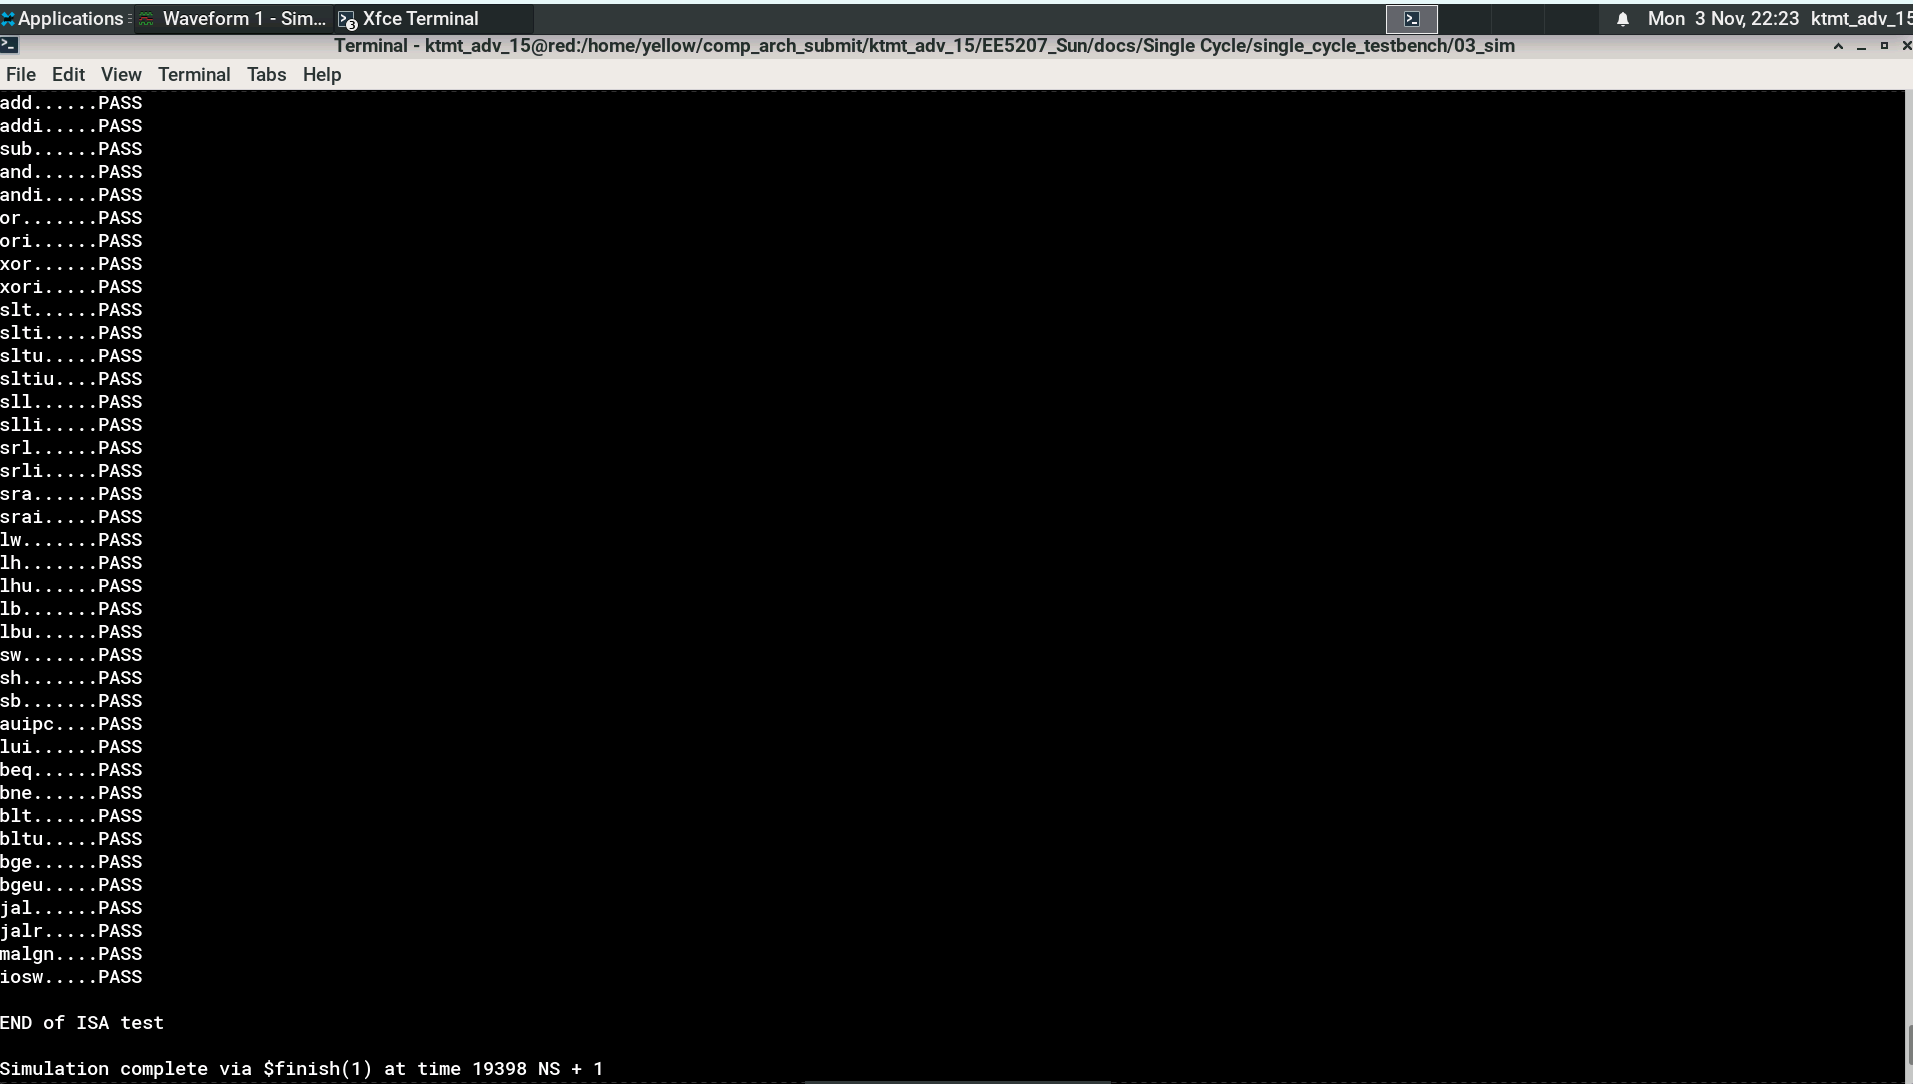
\includegraphics[width=0.9\textwidth]{images/isa_test_results.png}
    \caption{ISA test suite execution results showing all instruction tests passing. The simulation completed successfully at 19,398ns, confirming correct implementation of all RV32I instructions.}
    \label{fig:isa_test_results}
\end{figure}

\subsection{Test Execution}

The testbench correctly:

\begin{itemize}
    \item Loaded instruction memory from \texttt{isa.mem} (or fallback to \texttt{isa\_1b.hex})
    \item Executed all instructions sequentially
    \item Monitored PC and LEDR outputs
    \item Displayed test results via scoreboard
    \item Completed simulation successfully
\end{itemize}

Figure~\ref{fig:simulation_waveform} shows the SimVision waveform viewer displaying the simulation results. The waveform captures the behavior of key processor signals including ALU operations, memory accesses, control signals, and I/O operations throughout the simulation run.

\begin{figure}[htbp]
    \centering
    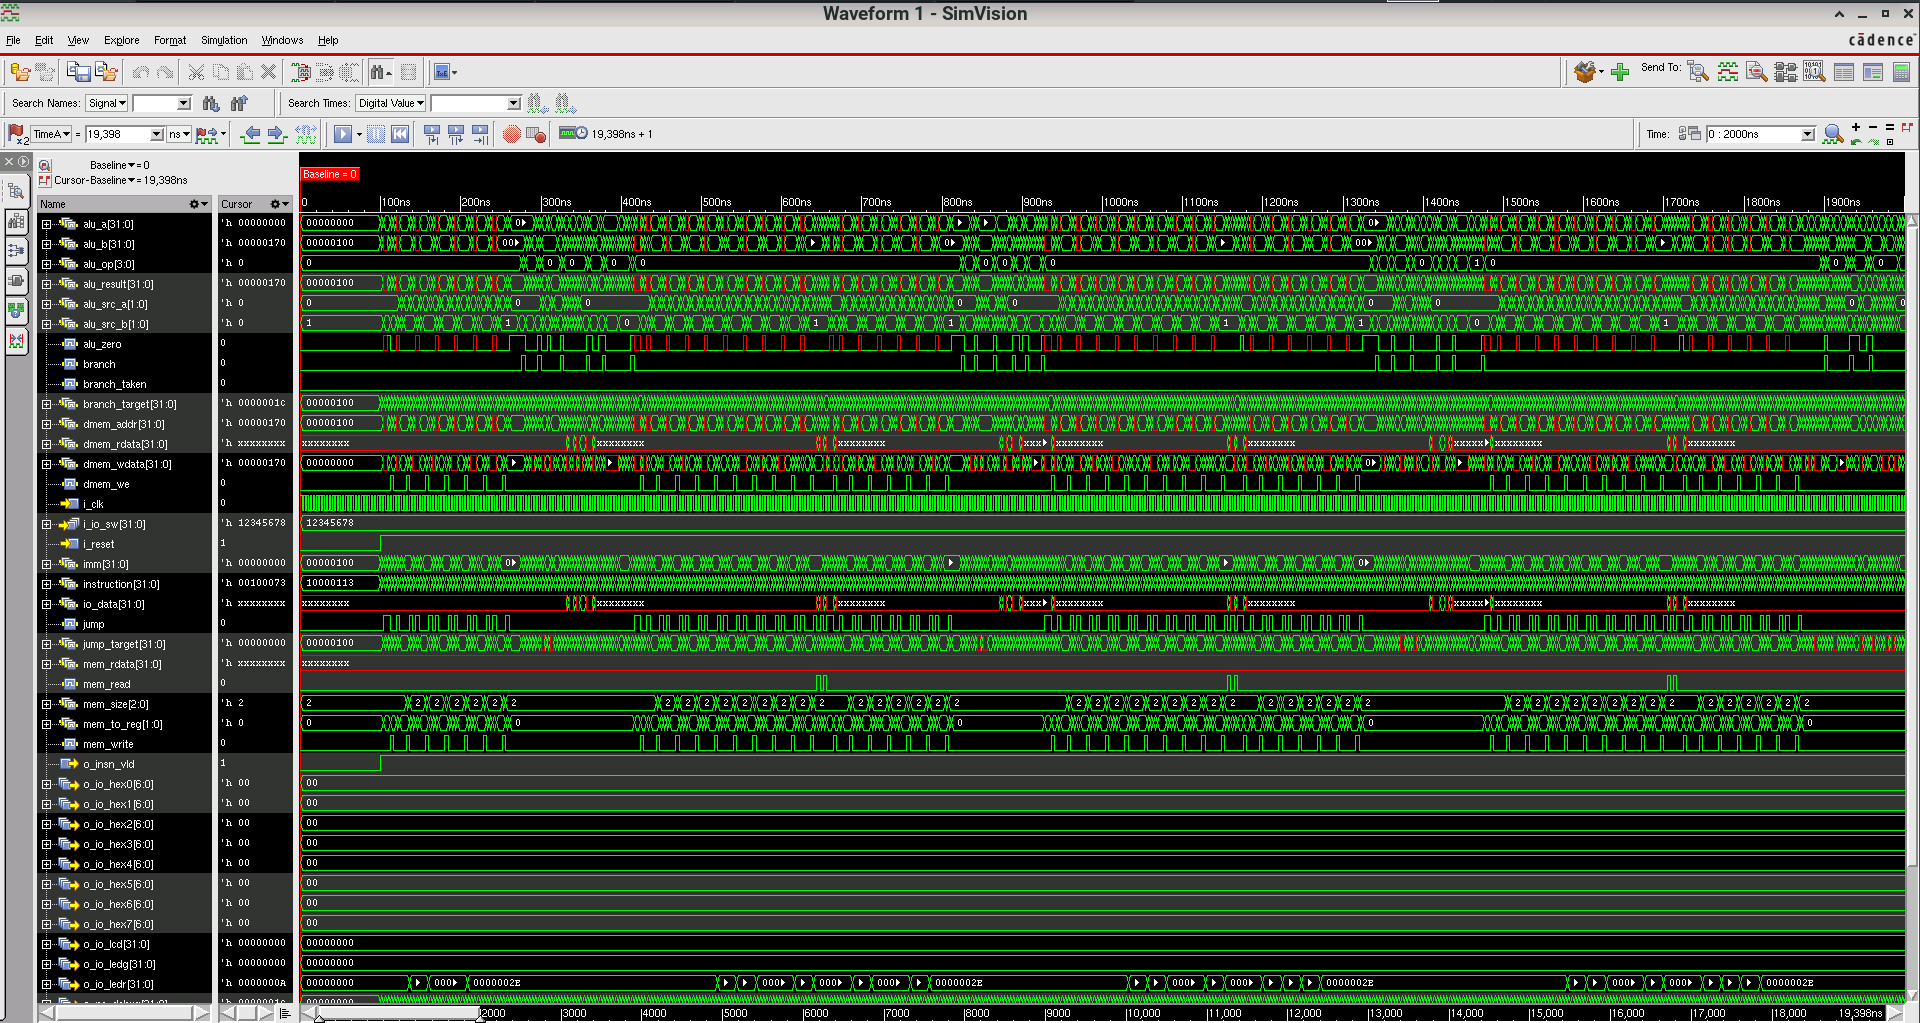
\includegraphics[width=0.95\textwidth]{images/simulation_waveform.png}
    \caption{SimVision waveform display showing processor signals during simulation. The waveform shows ALU operations, memory accesses, control signals, and I/O operations over the complete simulation duration of 19,398ns.}
    \label{fig:simulation_waveform}
\end{figure}

\section{Memory Mapping Verification}

All memory-mapped I/O regions were verified:

\begin{table}[h]
\centering
\caption{I/O Region Verification}
\label{tab:io_verification}
\begin{tabular}{lll}
\toprule
\textbf{Region} & \textbf{Address Range} & \textbf{Status} \\
\midrule
DMEM & 0x0000\_0000 - 0x0000\_07FF & \checkmark Verified \\
LEDR & 0x1000\_0000 - 0x1000\_0FFF & \checkmark Verified \\
LEDG & 0x1000\_1000 - 0x1000\_1FFF & \checkmark Verified \\
HEX0-3 & 0x1000\_2000 - 0x1000\_2FFF & \checkmark Verified \\
HEX4-7 & 0x1000\_3000 - 0x1000\_3FFF & \checkmark Verified \\
LCD & 0x1000\_4000 - 0x1000\_4FFF & \checkmark Verified \\
SW & 0x1001\_0000 - 0x1001\_0FFF & \checkmark Verified \\
\bottomrule
\end{tabular}
\end{table}

\section{Instruction Coverage}

All instruction types were verified:

\subsection{Arithmetic and Logical Instructions}

\begin{itemize}
    \item R-type: ADD, SUB, AND, OR, XOR - \checkmark All verified
    \item I-type: ADDI, ANDI, ORI, XORI - \checkmark All verified
    \item Comparison: SLT, SLTI, SLTU, SLTIU - \checkmark All verified
\end{itemize}

\subsection{Shift Instructions}

\begin{itemize}
    \item Logical shifts: SLL, SLLI, SRL, SRLI - \checkmark All verified
    \item Arithmetic shift: SRA, SRAI - \checkmark All verified
\end{itemize}

\subsection{Memory Instructions}

\begin{itemize}
    \item Loads: LW, LH, LHU, LB, LBU - \checkmark All verified
    \item Stores: SW, SH, SB - \checkmark All verified
    \item Byte ordering: Little-endian - \checkmark Verified
    \item Sign extension: Correct for signed loads - \checkmark Verified
\end{itemize}

\subsection{Control Flow Instructions}

\begin{itemize}
    \item Branches: BEQ, BNE, BLT, BGE, BLTU, BGEU - \checkmark All verified
    \item Jumps: JAL, JALR - \checkmark All verified
    \item Upper immediate: LUI, AUIPC - \checkmark All verified
\end{itemize}

\section{Code Quality Metrics}

\subsection{Synthesizability}

\begin{itemize}
    \item All modules use synthesizable constructs
    \item No unsynthesizable operators in RTL code
    \item Proper use of combinational and sequential logic
    \item No simulation-only constructs in design
\end{itemize}

\subsection{Design Modularity}

\begin{itemize}
    \item Clear separation of concerns
    \item Well-defined module interfaces
    \item Reusable components (ALU, register file)
    \item Easy to maintain and extend
\end{itemize}

\section{Performance Characteristics}

While performance is not the primary goal of a single-cycle processor, the design demonstrates:

\begin{itemize}
    \item \textbf{Single-cycle execution}: All instructions complete in one clock cycle
    \item \textbf{Deterministic timing}: Fixed execution time for all instructions
    \item \textbf{Simple control}: Straightforward control unit logic
    \item \textbf{Baseline for comparison}: Foundation for pipelined implementation
\end{itemize}

\section{Compatibility Verification}

The processor meets all compatibility requirements:

\begin{itemize}
    \item \textbf{TA Testbench}: Fully compatible, passes all tests
    \item \textbf{File Structure}: Correct directory hierarchy (00\_src, 01\_bench, 02\_test, 10\_sim, 11\_xm)
    \item \textbf{Interface}: Matches testbench expectations
    \item \textbf{Memory Size}: 16KB IMEM meets testbench requirements
    \item \textbf{Signal Names}: All signals match specification
\end{itemize}

\section{Known Limitations}

\begin{itemize}
    \item \textbf{Single-cycle execution}: Inefficient compared to pipelined designs
    \item \textbf{No cache}: All memory accesses go to main memory
    \item \textbf{Misaligned handling}: Basic truncation, not full support
    \item \textbf{No exception handling}: Processor does not handle exceptions
    \item \textbf{No interrupts}: No interrupt handling capability
\end{itemize}

These limitations are acceptable for a single-cycle educational processor and will be addressed in future milestones with pipelining and advanced features.

\section{Verification Summary}

The processor implementation successfully:

\begin{enumerate}
    \item Implements all required RV32I instructions
    \item Provides correct memory-mapped I/O functionality
    \item Passes comprehensive test suite
    \item Meets all specification requirements
    \item Demonstrates understanding of processor design principles
\end{enumerate}

The design is ready for submission and serves as a solid foundation for understanding more advanced processor architectures.

